
%(BEGIN_QUESTION)
% Copyright 2011, Tony R. Kuphaldt, released under the Creative Commons Attribution License (v 1.0)
% This means you may do almost anything with this work of mine, so long as you give me proper credit

Anta at du gjorde en god jobb med å montere en posisjoner på en reguleringsventil, inkludert nøye innretting av tilbakekoblingsmekanismen der posisjoneren kobles til ventilspindelen. Etter at du var ferdig, ble ventilen imidlertid overtatt av en person som ikke kunne noe om posisjonere. Vedkommende feiljusterte mekanismen mellom posisjoneren og ventilspindelen, ved å flytte vandringspinnen til en ny posisjon (høyere opp enn den skulle vært). Sammenlign illustrasjonene under som viser ``før-og-etter'':

$$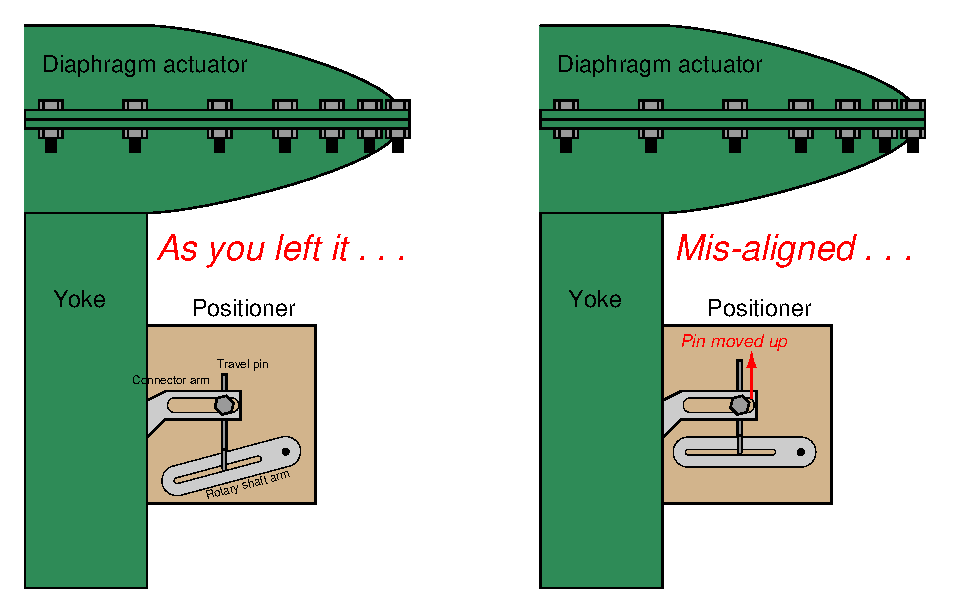
\includegraphics[width=15.5cm]{i01448x01.eps}$$

\noindent
Studer disse to illustrasjonene, og svar deretter på følgende spørsmål:

\begin{itemize}
\item{} Hvis tidligere kalibrering av denne posisjoneren var 4 mA (helt stengt) til 20 mA (helt åpen), velg det mest sannsynlige kalibreringsområdet ventilen nå har:
\begin{itemize}

\item{} Stengt ved 2 mA, helt åpen ved 22 mA
\item{} Stengt ved 6 mA, helt åpen ved 22 mA
\item{} Stengt ved 6 mA, helt åpen ved 18 mA
\vskip 10pt
\item{} Forklar hvorfor denne kalibreringsfeilen forårsaket av feilinnrettet mekanisme ikke kan korrigeres bare ved å justere null- og/eller span-innstillingene på posisjoneren. Med andre ord: Hvilke problemer vil fortsatt være til stede selv etter ny null- og span-justering (uten å justere mekanismen tilbake riktig)?
\end{itemize}
\end{itemize}

\underbar{file i01448}
%(END_QUESTION)





%(BEGIN_ANSWER)

Halv uttelling for hvert riktig svar:

\vskip 10pt

\begin{itemize}
\item{} {\bf Stengt ved 6 mA, helt åpen ved 22 mA}
\end{itemize}

\vskip 10pt

Denne feiljusteringen av tilbakekoblingsarmen vil gi flere problemer. Gi uttelling for {\it hvilket som helst} av svarene under, eller andre gyldige konklusjoner studenten kommer frem til:

\begin{itemize}
\item{} Selv etter ny null- og span-justering vil ventilen ikke lenger respondere {\it lineært}, fordi startvinkelen er feil.
\item{} Posisjonerarmens tillatte vandring vil sannsynligvis overskrides når ventilen går til helt åpen posisjon. Dette kan skade posisjoneren, og også gi ustabil ventiloppførsel nær fullt åpen posisjon.
\end{itemize}


%(END_ANSWER)





%(BEGIN_NOTES)

{\bf Dette spørsmålet er ment for eksamen og ikke arbeidsark!}.

%(END_NOTES)

